For the second iteration was the goal to remove the raycasting which that happens on runtime.

\subsection*{Minimizing the Graph size}
It was possible to reduce the number of waypoints even further.
To do so all waypoints are looped through to find adjacent waypoints, meaning waypoints whose distance to each other is less or equal to one.
Those that are adjacent are then removed and a new waypoint is placed halfway between them.
This is illustrated in Figure \ref{waypointMerge}.
The resulting waypoints can be seen in Figure \ref{waypointOpt} with the graph in Figure \ref{waypointgraphOpt}.
Most notably, the amount of edges are significantly reduced.
\begin{figure}[H]
	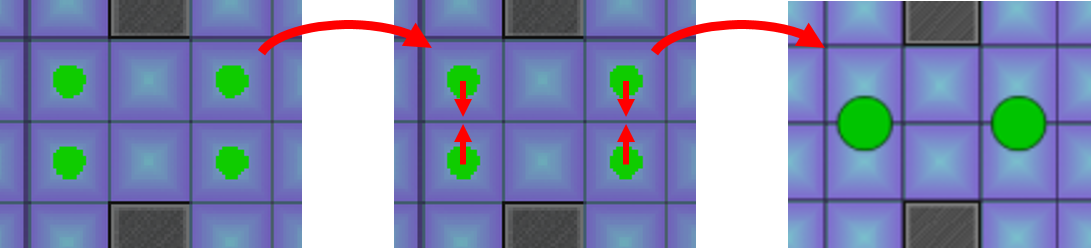
\includegraphics[width=\textwidth]{figures/astar/waypointMerge}
	\caption{Waypoint merging}
	\label{waypointMerge}
\end{figure}

\begin{figure}[H]
	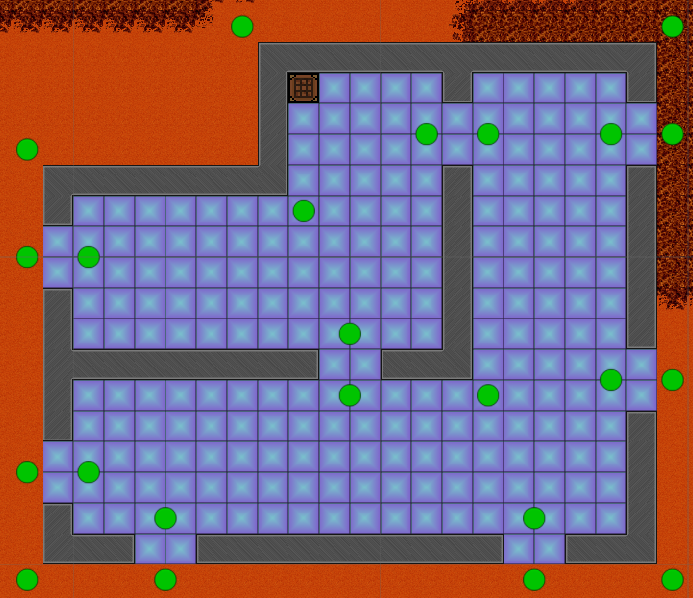
\includegraphics[width=\textwidth]{figures/astar/optimizedWaypoints}
	\caption{Waypoints after optimizations}
	\label{waypointOpt}
\end{figure}

\begin{figure}[H]
	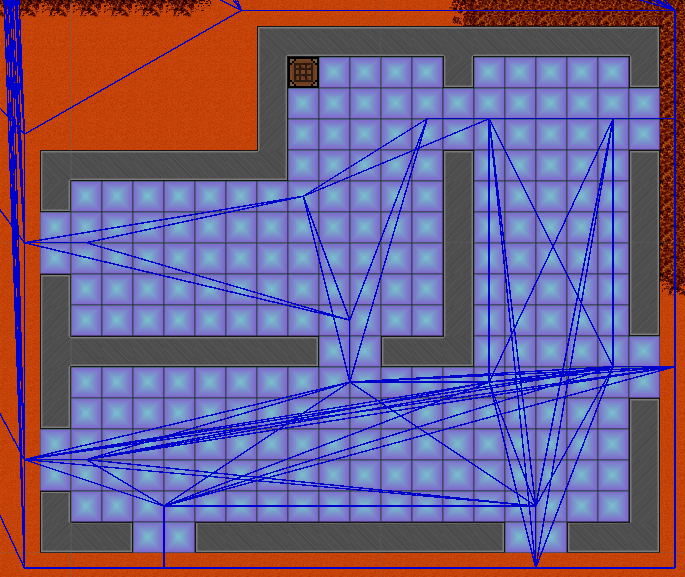
\includegraphics[width=\textwidth]{figures/astar/optimizedWaypointsGraph}
	\caption{Graph based on the waypoints after waypoint optimization}
	\label{waypointgraphOpt}
\end{figure}

\subsection*{Removing raycasts}
Raycast, in our case, is used to test if another object is accessible in a straight line.
The check 